\documentclass[11pt]{report}

% ---------------------------------------------------------------------------
% Packages
% ---------------------------------------------------------------------------
\usepackage[utf8]{inputenc}
\usepackage[T1]{fontenc}
\usepackage[a4paper,margin=2.5cm,headsep=14pt]{geometry}
\usepackage{textcomp}
\usepackage{xcolor}
\usepackage{tcolorbox}
\tcbuselibrary{skins,breakable}
\usepackage{tikz}
\usetikzlibrary{positioning,arrows.meta,shapes.geometric,fit,backgrounds}
\usepackage{listings}
\usepackage{longtable}
\usepackage{booktabs}
\usepackage{array}
\usepackage{enumitem}
\usepackage{titlesec}
\usepackage{fancyhdr}
\usepackage{parskip}
\usepackage{caption}
\usepackage{amssymb}
\usepackage{ragged2e}
\usepackage{lmodern}
\usepackage[final]{microtype}
\usepackage[colorlinks=true,linkcolor=svwlinkcolor,urlcolor=svwlinkcolor,citecolor=svwlinkcolor,bookmarksnumbered=true]{hyperref}

% ---------------------------------------------------------------------------
% Brand palette (lifted from app/static/index.html's Tailwind config)
% ---------------------------------------------------------------------------
\definecolor{svwdark}{HTML}{1A1C1E}
\definecolor{svwprimary}{HTML}{CD7F32}
\definecolor{svwaccent}{HTML}{E9C176}
\definecolor{svwlinkcolor}{HTML}{8A4B14}
\definecolor{bizboxbg}{HTML}{FFF6EA}
\definecolor{bizboxframe}{HTML}{CD7F32}
\definecolor{engboxbg}{HTML}{EAF1FB}
\definecolor{engboxframe}{HTML}{2C5C8A}
\definecolor{codebg}{HTML}{F7F7F7}
\definecolor{codeframe}{HTML}{CCCCCC}

% ---------------------------------------------------------------------------
% Callout boxes: bizbox = plain-English / commercial framing,
% engbox = engineering detail. Used throughout so both audiences can
% navigate the same document without reading it cover to cover.
% ---------------------------------------------------------------------------
\newtcolorbox{bizbox}[1][]{%
  enhanced, breakable, colback=bizboxbg, colframe=bizboxframe,
  boxrule=0.6pt, arc=2mm, left=6pt, right=6pt, top=5pt, bottom=5pt,
  fonttitle=\bfseries\sffamily\small, coltitle=svwdark,
  title={\textcolor{bizboxframe}{\textbullet}~~BUSINESS TAKEAWAY},#1}

\newtcolorbox{engbox}[1][]{%
  enhanced, breakable, colback=engboxbg, colframe=engboxframe,
  boxrule=0.6pt, arc=2mm, left=6pt, right=6pt, top=5pt, bottom=5pt,
  fonttitle=\bfseries\sffamily\small, coltitle=svwdark,
  title={\textcolor{engboxframe}{\textbullet}~~ENGINEERING NOTE},#1}

\newtcolorbox{qabox}[1]{%
  enhanced, breakable, colback=white, colframe=black!40,
  boxrule=0.4pt, arc=1mm, left=6pt, right=6pt, top=5pt, bottom=5pt,
  fonttitle=\bfseries, coltitle=svwdark,
  attach boxed title to top left={yshift=-2mm,xshift=4mm},
  boxed title style={colback=svwaccent!60,boxrule=0pt,arc=1mm},
  title={#1}}

% ---------------------------------------------------------------------------
% Code listings
% ---------------------------------------------------------------------------
\lstdefinestyle{base}{
  basicstyle=\ttfamily\scriptsize,
  commentstyle=\color{black!50}\itshape,
  stringstyle=\color{teal!70!black},
  keywordstyle=\color{svwlinkcolor}\bfseries,
  numbers=left, numberstyle=\tiny\color{black!40}, numbersep=8pt,
  breaklines=true, breakatwhitespace=false,
  frame=single, rulecolor=\color{codeframe}, framesep=4pt,
  backgroundcolor=\color{codebg},
  tabsize=2, showstringspaces=false,
  literate={£}{{\textsterling}}1 {≥}{{$\geq$}}1 {≤}{{$\leq$}}1,
  xleftmargin=2pt, xrightmargin=2pt,
}
\lstdefinestyle{py}{style=base, language=Python}
\lstdefinestyle{sql}{style=base, language=SQL}
\lstdefinestyle{plain}{style=base, language=}

% Inline code: \code{...} avoids underscore-escaping headaches.
\newcommand{\code}[1]{\lstinline[style=plain]!#1!}
% \codeb{...}: for long identifiers that must be allowed to break across a
% line (lstinline never breaks); content must use \_ for underscores and
% may include \allowbreak{} at a sensible split point.
\newcommand{\codeb}[1]{\texttt{\scriptsize #1}}

% ---------------------------------------------------------------------------
% Headings / headers
% ---------------------------------------------------------------------------
\titleformat{\chapter}[display]
  {\bfseries\sffamily}{\Large\textcolor{svwprimary}{Chapter \thechapter}}{4pt}{\Huge}
\titlespacing*{\chapter}{0pt}{0pt}{20pt}
\titleformat{\section}{\bfseries\sffamily\Large\color{svwdark}}{\thesection}{8pt}{}
\titleformat{\subsection}{\bfseries\sffamily\large\color{svwdark}}{\thesubsection}{8pt}{}

\pagestyle{fancy}
\fancyhf{}
\renewcommand{\headrulewidth}{0.4pt}
\fancyhead[L]{\footnotesize\sffamily\textcolor{black!50}{\leftmark}}
\fancyhead[R]{\footnotesize\sffamily\textcolor{black!50}{WealthLink}}
\fancyfoot[C]{\small\thepage}
\renewcommand{\chaptermark}[1]{\markboth{\textsc{Chapter \thechapter} ---  #1}{}}

\setlength{\parskip}{6pt}
\setlist{itemsep=2pt, topsep=4pt}

\hypersetup{
  pdftitle={Single View of Wealth -- Technical and Commercial Reference},
  pdfauthor={WealthLink SVW Project},
  pdfsubject={Entity Resolution Proof of Concept},
}

% ---------------------------------------------------------------------------
\begin{document}

% =============================================================================
% TITLE PAGE
% =============================================================================
\begin{titlepage}
\begin{tikzpicture}[remember picture, overlay]
  \fill[svwdark] (current page.north west) rectangle ([yshift=-7cm]current page.north east);
  \node[anchor=north west, text=svwaccent, font=\sffamily\bfseries\Huge, align=left]
    at ([xshift=2cm,yshift=-2.2cm]current page.north west) {WealthLink};
  \node[anchor=north west, text=white, font=\sffamily\large, align=left]
    at ([xshift=2cm,yshift=-3.7cm]current page.north west) {Single View of Wealth Platform};
  \node[anchor=north west, text=white!70!black, font=\sffamily\small, align=left]
    at ([xshift=2cm,yshift=-4.5cm]current page.north west) {Entity-resolution proof of concept for a multi-subsidiary banking group};
\end{tikzpicture}
\vspace*{8.2cm}

\begin{center}
{\sffamily\bfseries\Large Technical \& Commercial Reference}\\[6pt]
{\sffamily\large\color{black!60} How the demo works, why it was built this way, and how to present and defend it}\\[24pt]
\end{center}

\vspace{1.5cm}
\begin{center}
\begin{tcolorbox}[width=0.85\textwidth, colback=bizboxbg, colframe=bizboxframe, arc=2mm, boxrule=0.6pt]
\centering
\textbf{Who this document is for}\\[4pt]
\footnotesize
\textbf{Sales \& presales teams} get a plain-English walkthrough of the problem, the demo, and the pitch.\\
\textbf{Engineers \& solution architects} get a module-by-module technical breakdown, the entity-resolution methodology, the data model, the API surface, and a prepared FAQ for technical due diligence.\\
Look for the \textcolor{bizboxframe}{\textbf{orange}} boxes for business framing and the \textcolor{engboxframe}{\textbf{blue}} boxes for engineering depth.
\end{tcolorbox}
\end{center}

\vfill
\begin{center}
\footnotesize\color{black!50}
Document generated from the \texttt{SCV} repository (\texttt{app/}, \texttt{demo.py}, \texttt{README.md}).\\
Project status: \textbf{Proof of Concept} --- not production-hardened. See Chapter~\ref{ch:limitations}.\\
Generated \today.
\end{center}
\end{titlepage}

\tableofcontents

% =============================================================================
\chapter{Executive Summary}
% =============================================================================

\textbf{Single View of Wealth (SVW)} is a working demonstration of how a banking group with several subsidiaries can stop treating each subsidiary's customer data as a separate island, and instead see \emph{one consolidated picture of wealth} for every individual across the whole group --- automatically, and without asking any subsidiary to change its own systems first.

The proof of concept (PoC) does three things end-to-end, live, in front of a viewer:

\begin{enumerate}
\item \textbf{Simulates the real problem.} It generates a realistic synthetic population of 10,000 people and ``leaks'' them across five fictional subsidiary banks as 25,000+ payroll records and tens of thousands of banking-product holdings (current accounts, savings, investments, mortgages) -- each subsidiary capturing the same person slightly differently (nicknames, typos, formatting differences, missing fields), exactly the way real organically-grown subsidiary IT estates do.
\item \textbf{Resolves identity.} It runs an industry-grade probabilistic record-linkage engine (\textbf{Splink}, the open-source entity-resolution library originally built by the UK Ministry of Justice) over every one of those noisy records and works out, statistically, which records belong to the same real person -- without ever being told the answer.
\item \textbf{Builds the golden record.} It aggregates every resolved person's salary, cash, savings, investments and mortgage balances into a single ``Single View of Wealth'' profile, complete with a wealth tier, a percentile ranking, and a transparent, field-by-field explanation of \emph{why} the system believes these records belong to the same person.
\end{enumerate}

All of this is wrapped in a polished web dashboard and a documented REST API, so it can be demoed live, explored by a technical evaluator, or scripted end-to-end from the command line (\texttt{demo.py}) with no server at all.

\begin{bizbox}
\textbf{Why a buyer should care.} Most banking groups grew by acquisition or by spinning up subsidiaries with their own core banking systems. None of them share a customer ID. The result: the group cannot answer simple questions like \emph{``what is our total relationship with this household?''}, cannot cross-sell effectively, under-prices risk, and struggles with KYC/AML obligations that require knowing who their customers really are across the whole group. This PoC proves, on realistic synthetic data, that the hard part -- resolving identity across messy, independently-captured records -- is solvable today, with mature open-source technology, in well under a minute, on a single laptop.
\end{bizbox}

\begin{engbox}
\textbf{What's genuinely real here vs.\ simulated.} The data is 100\% synthetic (Faker-generated, seeded for reproducibility) -- nothing here is a real customer. What \emph{is} real is the entity-resolution methodology: Splink's probabilistic (Fellegi--Sunter) matching model, trained with Expectation-Maximisation, scored and clustered exactly as it would be against production data. The PoC also keeps a hidden ``ground truth'' (which records really belong to which synthetic person) purely so it can measure its own precision/recall -- a luxury that disappears in production, where this same pipeline would run unchanged but unverified by ground truth.
\end{engbox}

% =============================================================================
\chapter{The Business Problem}
% =============================================================================

\section{Why subsidiaries can't see the whole customer}

Picture a banking group with five subsidiaries: a retail bank, a wealth manager, a trust company, a commercial bank, and a private bank. Each was built or bought at a different time, on different core banking software, with its own employee/payroll system and its own customer-onboarding process. None of them were ever designed to talk to each other, and none of them share a common customer or employee identifier.

When the same person -- say, a senior employee who also banks personally with two of the group's subsidiaries -- shows up in all five systems, each system has its own slightly different snapshot of who they are:

\begin{itemize}
\item One spells their name in full (\emph{Jonathan}), another uses a nickname (\emph{Jon}) or just an initial (\emph{J}).
\item One stores their address as ``10 Main Street'', another abbreviates it to ``10 Main St''.
\item One has their postcode with a space, another without.
\item Email addresses differ by format (\code{jon.smith@gmail.com} vs.\ \code{jsmith23@gmail.com}) because each subsidiary's onboarding form generated its own.
\item Fields are sometimes simply missing -- a phone number never captured, an address left blank.
\end{itemize}

\begin{bizbox}
None of this is a data-entry failure to be blamed on any one team. It is the \emph{normal, expected} state of any organisation that grew through multiple systems. The problem only becomes visible -- and costly -- when the group tries to answer a question that spans subsidiaries: ``how much does this person really hold with us, across everything?''
\end{bizbox}

\section{The cost of not solving it}

\begin{itemize}
\item \textbf{Missed commercial opportunity.} A private banking subsidiary cannot identify that one of its high-net-worth clients is also a payroll-earning senior employee at the group's commercial bank -- a natural cross-sell and relationship-pricing opportunity that simply never surfaces.
\item \textbf{Mispriced risk.} Credit and exposure decisions made subsidiary-by-subsidiary underestimate a customer's true indebtedness or overstate their true liquidity, because no single view of their mortgage, savings and investment position exists.
\item \textbf{Regulatory and KYC/AML exposure.} ``Know Your Customer'' and anti-money-laundering obligations increasingly expect a group-wide view of a customer relationship, not five fragmented ones. Failing to produce one is a genuine compliance and audit finding waiting to happen.
\item \textbf{Poor customer experience.} Customers experience the group as five unconnected companies, repeating the same information five times, with no acknowledgement that the bank already knows them elsewhere in the group.
\end{itemize}

\section{Why this is hard, not just tedious}

The obvious-sounding fix -- ``just match the records where the names and addresses are the same'' -- breaks immediately on real data, because real data never matches \emph{exactly}. ``Jon Smith, 10 Main St'' and ``Jonathan Smith, 10 Main Street'' are clearly the same person to a human reader, but an exact-match SQL \code{JOIN} sees two completely unrelated strings. Scaling that judgement call to hundreds of thousands of records, consistently and auditably, is what this PoC exists to prove is achievable.

\begin{bizbox}
This is the industry problem usually called building a \textbf{Single Customer View} or a \textbf{golden record}. It is a well-trodden, well-understood data-management discipline -- this PoC demonstrates it can be stood up quickly, cheaply, and transparently, using mature open-source tooling rather than a multi-year, multi-million-pound master-data-management programme.
\end{bizbox}

% =============================================================================
\chapter{How the Solution Works, in Plain English}
% =============================================================================

\section{The pipeline at a glance}

The platform is a four-stage pipeline. Figure~\ref{fig:pipeline} shows the flow; each stage is a Python module in the codebase, named for what it does.

\begin{figure}[h]
\centering
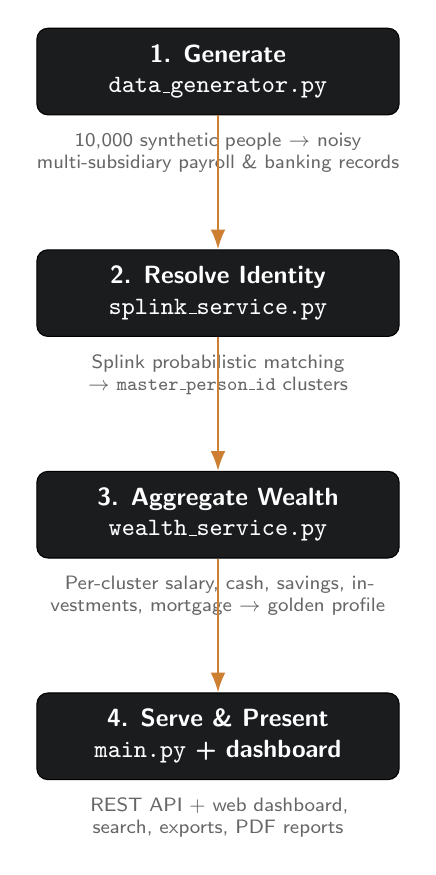
\begin{tikzpicture}[
  node distance=0.9cm,
  box/.style={draw, rounded corners, fill=svwdark, text=white, font=\sffamily\small\bfseries, minimum width=4.6cm, minimum height=1.1cm, align=center},
  lbl/.style={font=\sffamily\scriptsize, text=black!60, align=center, text width=4.6cm},
  arr/.style={-{Latex[length=2.5mm]}, thick, color=svwprimary}
]
\node[box] (gen) {1. Generate\\ \texttt{data\_generator.py}};
\node[lbl, below=1mm of gen] (genl) {10,000 synthetic people $\rightarrow$ noisy multi-subsidiary payroll \& banking records};

\node[box, below=1.7cm of gen] (link) {2. Resolve Identity\\ \texttt{splink\_service.py}};
\node[lbl, below=1mm of link] (linkl) {Splink probabilistic matching $\rightarrow$ \texttt{master\_person\_id} clusters};

\node[box, below=1.7cm of link] (wealth) {3. Aggregate Wealth\\ \texttt{wealth\_service.py}};
\node[lbl, below=1mm of wealth] (wealthl) {Per-cluster salary, cash, savings, investments, mortgage $\rightarrow$ golden profile};

\node[box, below=1.7cm of wealth] (api) {4. Serve \& Present\\ \texttt{main.py} + dashboard};
\node[lbl, below=1mm of api] (apil) {REST API + web dashboard, search, exports, PDF reports};

\draw[arr] (gen) -- (link);
\draw[arr] (link) -- (wealth);
\draw[arr] (wealth) -- (api);
\end{tikzpicture}
\caption{The end-to-end SVW pipeline. Every stage persists its output to a single embedded DuckDB database file (\texttt{data/svow.duckdb}), so each stage can be re-run independently.}
\label{fig:pipeline}
\end{figure}

\section{Stage 1: Simulating the problem}

Rather than risk (or need) real customer data, the PoC generates its own realistic population using \textbf{Faker}, a library that produces plausible-looking but entirely fictional names, addresses, emails and dates. It then simulates, in software, exactly the kind of imperfect data capture described in Chapter~2: nicknames, abbreviated addresses, reformatted phone numbers, missing fields, and so on. Every run uses the same random seed, so the same demo always produces the same (impressive) results.

\section{Stage 2: Resolving identity (entity resolution)}

This is the heart of the product. Think of it like a very careful detective comparing thousands of slightly different witness statements and working out which ones describe the same person. The system looks at every pair of records that could plausibly be the same person and asks, field by field: \emph{do the names sound alike? Is the date of birth close? Does the postcode match? Does the email share a username?} It then combines all of these clues into a single confidence score between 0\% and 100\%.

Records whose confidence score clears a chosen bar are linked together into a group representing one real person, given a new shared ID (\code{master_person_id}, e.g.\ \code{MP00001}). This is exactly what a human analyst would do manually, given unlimited time -- the system just does it for tens of thousands of records in under a minute, consistently, and shows its working.

\begin{bizbox}
This is the single most valuable and most defensible part of the demo. It is powered by \textbf{Splink}, an open-source entity-resolution engine originally developed by the UK Ministry of Justice and now widely used across UK government and industry. It is not a black box or a toy fuzzy-matching script -- it is the same statistical methodology (Fellegi--Sunter probabilistic record linkage) used in production data-linkage systems handling tens of millions of records.
\end{bizbox}

\section{Stage 3: Building the golden Single View of Wealth}

Once the system knows which records belong to the same person, it combines their financial information into one profile:

\begin{itemize}
\item \textbf{Salary} is averaged across that person's linked payroll records (each subsidiary's payroll feed is recording the same job, so averaging smooths small reporting differences rather than double-counting).
\item \textbf{Cash, savings, investments and mortgage balances} are summed, because someone can genuinely hold several real accounts of the same type across different subsidiaries, and each one is real wealth or real debt.
\item \textbf{Net wealth} is cash + savings + investments minus mortgage debt.
\end{itemize}

Every resolved person is then ranked against everyone else in the bank's population and assigned a wealth percentile and a simple commercial segment label (Mass Market, Affluent, High Net Worth, Ultra High Net Worth, or Negative Equity) -- the kind of segmentation a private bank or wealth manager already uses to decide who gets a relationship manager call.

\section{Stage 4: The dashboard --- what you actually see in a demo}

The dashboard (Figure~\ref{fig:dashboard-tour}, described below) is what gets shown in a sales meeting. It has four views:

\begin{description}
\item[Dashboard] Headline KPIs (population, total records, resolved clusters, duplicates found, average match confidence, total net wealth under management), and the centrepiece: an \textbf{``Entity Resolution In Action''} panel that shows one real resolved person exactly as their records looked \emph{before} the system ran (several records that look like different people) and \emph{after} (one consolidated profile) -- pulled live from whatever the current run produced, not a canned screenshot.
\item[Directory] A searchable list of every resolved person, with the option to export the whole list as CSV.
\item[Profile] A single person's full dossier: their wealth breakdown, every linked source record with its own confidence score, and a ``Match Explanation'' panel that says, in plain language, exactly which fields agreed across the linked records and which ones still disagree (e.g.\ two different postcodes were seen). This is what makes the system's reasoning auditable rather than a black box.
\item[Data Quality] A transparency page: a histogram of how confident the system was across the whole population, a breakdown of cluster sizes, and a ``manual review queue'' of the handful of lowest-confidence matches a real bank's analyst team would want to sanity-check by hand.
\end{description}

\begin{bizbox}
\textbf{The demo's best moment} is the Dashboard's before/after panel: showing a viewer several records that visibly look like different people (different name spellings, different contact details) and then showing the single consolidated profile the system produced from them, with a confidence score attached to every link. It turns an abstract claim (``we do entity resolution'') into a concrete, visual, two-second ``aha''.
\end{bizbox}

\begin{figure}[h]
\centering
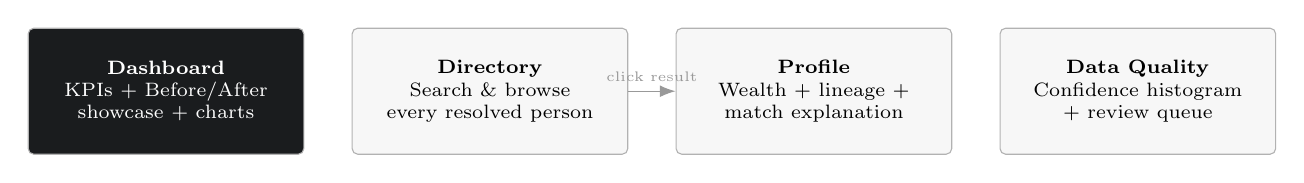
\begin{tikzpicture}[
  node distance=6mm,
  card/.style={draw=black!30, rounded corners=2pt, fill=black!3, minimum width=3.5cm, minimum height=1.6cm, align=center, font=\scriptsize},
]
\node[card, fill=svwdark, text=white] (dash) {\textbf{Dashboard}\\KPIs + Before/After\\showcase + charts};
\node[card, right=of dash] (dir) {\textbf{Directory}\\Search \& browse\\every resolved person};
\node[card, right=of dir] (prof) {\textbf{Profile}\\Wealth + lineage +\\match explanation};
\node[card, right=of prof] (qual) {\textbf{Data Quality}\\Confidence histogram\\+ review queue};
\draw[-{Latex[length=2mm]}, color=black!40] (dir) -- node[above,font=\tiny]{click result} (prof);
\end{tikzpicture}
\caption{The four views of the WealthLink dashboard (\texttt{app/static/}), all backed live by the JSON API -- nothing on screen is hardcoded.}
\label{fig:dashboard-tour}
\end{figure}

\section{The five-minute live demo script}

The repository includes \texttt{demo.py}, a self-contained command-line script with no server required, designed to be run live:

\begin{enumerate}
\item Generates the synthetic dataset.
\item Picks one person who has noisy records across at least three subsidiaries and prints them -- visibly looking like different people.
\item Runs the full Splink pipeline.
\item Prints the resolved \code{master_person_id}, every subsidiary that was linked to it, and each link's confidence score.
\item Prints that person's final Single View of Wealth: salary, cash, savings, investments, mortgage, and net wealth.
\end{enumerate}

\begin{bizbox}
This script is the fastest way to demonstrate the core value proposition to a non-technical stakeholder without touching a browser: run one command, watch ``five different people'' become ``one person, with a complete financial picture'', in well under a minute.
\end{bizbox}

% =============================================================================
\chapter{Architecture Overview}
\label{ch:architecture}
% =============================================================================

\section{Technology stack}

\begin{table}[h]
\centering
\small
\begin{tabular}{@{}p{3.6cm}p{9.5cm}@{}}
\toprule
\textbf{Component} & \textbf{Role} \\
\midrule
FastAPI & Python web framework serving the REST API and the static dashboard. \\
DuckDB & Embedded, file-based analytical database (\texttt{data/svow.duckdb}); no separate database server to install or operate. \\
Splink (DuckDB backend) & Probabilistic record-linkage / entity-resolution engine -- the core IP of the demo. \\
Faker & Synthetic data generator (names, addresses, emails, phone numbers, dates). \\
Pandas / NumPy & In-memory data manipulation between generation, linkage and persistence steps. \\
PyJWT + bcrypt & JSON Web Token issuing/verification and password hashing for the login layer. \\
ReportLab & Server-side PDF rendering for the profile export report. \\
Tailwind CSS (CDN) + Chart.js (CDN) & Dependency-free, build-step-free dashboard frontend (plain HTML/JS). \\
\bottomrule
\end{tabular}
\caption{Full technology stack. Everything runs in a single process with no external services -- deliberately, so the whole PoC is one \texttt{uvicorn} command.}
\end{table}

\begin{engbox}
Every dependency is pinned to a version range in \texttt{app/requirements.txt}. There are no calls to external APIs or cloud services anywhere in the codebase -- the entire pipeline, from synthetic data generation to PDF export, runs fully offline.
\end{engbox}

\section{Module map}

\begin{longtable}{@{}p{3.6cm}p{9.7cm}@{}}
\toprule
\textbf{Module} & \textbf{Responsibility} \\
\midrule
\endhead
\texttt{data\_generator.py} & Seeded synthetic data generation: people, noisy multi-subsidiary payroll records, and noisy banking-product records, all persisted into one unified \texttt{records} table. \\
\texttt{models.py} & Internal domain models (Pydantic) describing each DuckDB table's row shape. \\
\texttt{splink\_service.py} & Splink configuration and the train $\to$ predict $\to$ cluster pipeline. \\
\texttt{wealth\_service.py} & Aggregates clusters into wealth profiles; powers search, dashboard and data-quality queries. \\
\texttt{auth.py} & JWT login, password hashing, and role-based access control. \\
\texttt{exports.py} & CSV and PDF report rendering on top of \texttt{wealth\_service}'s existing queries. \\
\texttt{schemas.py} & Public API request/response contracts (Pydantic), independent of the internal storage shape. \\
\texttt{main.py} & FastAPI app wiring, startup auto-bootstrap, and every HTTP endpoint. \\
\texttt{static/index.html}, \texttt{static/app.js} & The dependency-free dashboard frontend, served at \texttt{/}. \\
\texttt{demo.py} & Standalone before/after CLI walkthrough; no server required. \\
\bottomrule
\caption{Module responsibilities. See Chapters~5--12 for a deep dive on each.}
\end{longtable}

\section{Why these particular technology choices}

\begin{description}[style=nextline]
\item[Why DuckDB, not Postgres/MySQL?] DuckDB is an embedded, file-based, single-process analytical database -- there is nothing to install, configure, or operate, and it is extremely fast for the bulk SQL aggregation this PoC does. \texttt{splink\_service.py} also uses Splink's native \texttt{DuckDBAPI} backend, so the entity-resolution engine and the storage layer share the same technology, keeping the whole stack to one moving part.
\item[Why Splink specifically?] Splink implements the Fellegi--Sunter probabilistic record-linkage model with a modern, well-tested API, purpose-built comparison functions for names/dates/emails/postcodes, and a scalable in-process execution engine (DuckDB, Spark, or Athena backends). It is open-source, actively maintained, and already proven at scale in government and industry deployments -- a far stronger foundation than a bespoke fuzzy-matching script.
\item[Why a build-step-free frontend?] The dashboard is plain HTML/JavaScript using Tailwind CSS and Chart.js from a CDN, with no bundler, framework, or \texttt{npm install} step. This keeps the entire PoC runnable from a single \texttt{uvicorn} command, which matters when the audience is a prospect's laptop in a meeting room, not a CI/CD pipeline.
\end{description}

% =============================================================================
\chapter{Technical Deep Dive: Synthetic Data Generation}
\label{ch:datagen}
% =============================================================================

\textit{Module: \texttt{app/data\_generator.py}}

\section{Purpose and reproducibility}

Because this is a PoC and no real customer data is available (or should be used), \texttt{data\_generator.py} builds an entirely synthetic but statistically realistic population, and then simulates how five independent subsidiary IT systems would \emph{imperfectly} capture that same population. Every random draw is seeded (\code{SEED = 777}), so the exact same dataset --- and therefore the exact same demo --- is produced on every machine, every time.

\begin{engbox}
Reproducibility is achieved with a dedicated \code{random.Random(seed)} instance threaded through every generation function (never the global \code{random} module), plus \code{Faker.seed(seed)} for the Faker-driven fields. This means two calls to \code{generate_all()} with the same seed are bit-for-bit identical, which is what lets the threshold-sweeping precision/recall analysis in Chapter~\ref{ch:splink} be trusted.
\end{engbox}

\section{Population and scale}

\begin{itemize}
\item \textbf{10,000} ground-truth people (\code{N_PEOPLE}), each independently generated by Faker's \code{en_GB} locale (UK-style names, addresses, postcodes, phone numbers), aged 21--66.
\item Each person is independently recorded by between 1 and 4 of the group's five subsidiaries' payroll systems, with an \emph{exact} target distribution (not just approximate): 2,000 people recorded by 1 subsidiary, 3,000 by 2, 3,000 by 3, and 2,000 by 4 -- totalling exactly \textbf{25,000} payroll records.
\item Each person is also independently assigned a banking-product ``bundle'' (payroll-only, payroll + deposits, payroll + investments, payroll + mortgage, or all products), which determines which of the four banking-product types (current account, savings, investment, mortgage) they hold, at which subsidiaries, and how many accounts of each.
\end{itemize}

The five subsidiaries are modelled as a Python enum (\texttt{app/models.py}) with both a display name and a short internal code:

\begin{lstlisting}[style=py, caption={The five subsidiaries (\texttt{app/models.py})}]
class Subsidiary(str, Enum):
    A = "Hawksworth Retail Bank"
    B = "Calder Wealth Partners"
    C = "Brightfield Trust"
    D = "Sterling Commercial Bank"
    E = "Ridgeway Private Bank"
\end{lstlisting}

\section{The noise model: simulating five imperfect subsidiary systems}

The same seven identity fields (first name, last name, date of birth, email, phone, address, postcode -- city is left untouched) are independently ``re-captured'' for every record, payroll or banking product alike, via one shared function, \code{_noisy_identity_capture()}. This guarantees the noise model is identical regardless of which kind of record is being generated, so Splink genuinely cannot use record type as a shortcut.

\begin{table}[h]
\centering
\small
\begin{tabular}{@{}p{3.2cm}p{9.9cm}@{}}
\toprule
\textbf{Field} & \textbf{Noise simulated} \\
\midrule
First name & 55\% unchanged; then a real nickname if one exists for that name (e.g.\ \emph{William} $\to$ \emph{Will}/\emph{Bill}/\emph{Billy}); then an initial only (\emph{W}); then a random upper/lower-case variant. \\
Last name & 85\% unchanged; then an upper/lower-case variant; then (rarely) a transposed-letter typo simulating a transcription error. \\
Date of birth & 95\% unchanged; 5\% has day and month transposed (a classic data-entry error, only when the day is $\leq$12 so it remains a valid date). \\
Address & Street-type tokens (\emph{Street}, \emph{Road}, \emph{Avenue}, \ldots) independently abbreviated (\emph{St}, \emph{Rd}, \emph{Ave}, \ldots) with 50\% probability per occurrence. \\
Postcode & 30\% chance the internal space is stripped (\texttt{TF2R 2LQ} $\to$ \texttt{TF2R2LQ}). \\
Email & 50\% chance of reusing the canonical address verbatim; otherwise regenerated under a different formatting convention (dot/no-dot/initial/underscore, different webmail domain, optional numeric suffix) -- simulating a different subsidiary's own account-issuing system. \\
Phone & 50\% chance of reuse verbatim; otherwise formatting characters (spaces, brackets, dashes) are stripped. \\
\midrule
Missing values & Independently, email is nulled 12\% of the time, phone 12\%, address 10\% -- fields simply never captured by that subsidiary. \\
\bottomrule
\end{tabular}
\caption{The full identity-noise model, applied identically to every payroll and banking-product record.}
\end{table}

\begin{bizbox}
These aren't arbitrary numbers -- they encode the exact failure modes a real bank's data-quality team will recognise immediately: nicknames, abbreviations, formatting drift, and missing fields. Showing a prospect this table is often more convincing than the demo itself, because it proves the PoC was built to mirror their actual data problem, not a sanitised toy version of it.
\end{bizbox}

\subsection{Worked example: \texttt{\_vary\_first\_name}}

\begin{lstlisting}[style=py, caption={Cumulative-threshold noise sampling (\texttt{data\_generator.py})}]
def _vary_first_name(first_name: str, rng: random.Random) -> str:
    key = first_name.lower()
    roll = rng.random()
    if roll < FIRST_NAME_UNCHANGED_PROB:        # 0.55
        return first_name
    if key in NICKNAMES and roll < FIRST_NAME_NICKNAME_PROB:   # 0.80
        return rng.choice(NICKNAMES[key])
    if roll < FIRST_NAME_INITIAL_PROB:          # 0.92
        return first_name[0]
    return first_name.upper() if rng.random() < 0.5 else first_name.lower()
\end{lstlisting}

\begin{engbox}
Note the thresholds are \emph{cumulative}, not independent per-branch probabilities -- a single \code{roll} is drawn once and compared against ascending thresholds in sequence. This is a common source of bugs if a future edit inserts a new branch without re-deriving the thresholds below it; the module-level constants are deliberately named for the branch they gate (e.g.\ \code{*_UNCHANGED_PROB}) so the intent is harder to invert by accident.
\end{engbox}

\section{Statistical realism: salaries, balances and mortgages}

A flat \code{uniform(low, high)} salary or balance would look obviously synthetic -- real income and wealth distributions are right-skewed, with most people sitting well below the maximum and a shrinking population stretching out toward it. The generator therefore uses a \textbf{shifted lognormal distribution}:

\begin{lstlisting}[style=py, caption={Shifted lognormal sampler (\texttt{data\_generator.py})}]
def _lognormal(rng, floor, median_above_floor, sigma, high):
    """floor + a lognormal-distributed excess over it, capped at high."""
    return min(high, floor + rng.lognormvariate(
        math.log(median_above_floor), sigma))
\end{lstlisting}

\begin{engbox}
Shifting (adding the lognormal excess \emph{on top of} a floor) rather than simply clamping a plain lognormal at the floor matters: clamping would pile up a visible spike of values sitting exactly on the floor in a histogram, which looks obviously synthetic. Shifting makes the floor smoothly unreachable, tapering down toward it instead -- indistinguishable from a real income/wealth histogram at a glance.
\end{engbox}

This same function (with different parameters) drives annual salary (floor \textsterling30,000, capped at \textsterling250,000), current-account balances (floor \textsterling50, capped at \textsterling50,000), savings (floor \textsterling200, capped at \textsterling200,000), and investments (floor \textsterling500, capped at \textsterling500,000). Bonuses use a \textbf{Beta(2,5)} distribution (skewed toward modest payouts, capped at 50\% of salary), and mortgage balances use a \textbf{triangular distribution} centred on a 3.5$\times$-salary affordability multiple (realistic UK mortgage-lending behaviour), clamped to \textsterling50,000--\textsterling600,000.

\begin{bizbox}
Net wealth is deliberately defined as cash + savings + investments $-$ mortgage, with no offsetting property-value asset. This means a customer with only payroll income and a mortgage will show a \emph{negative} net wealth figure on the dashboard -- this is by design (matching the agreed wealth formula), not a bug, and is worth pre-empting in a demo before a sharp-eyed viewer asks about it.
\end{bizbox}

\section{The unified \texttt{records} table}

Every kind of record -- payroll \emph{and} all four banking-product types -- is written into one table, distinguished by a \code{record_type} column (\code{PAYROLL}, \code{CURRENT_ACCOUNT}, \code{SAVINGS_ACCOUNT}, \code{INVESTMENT}, \code{MORTGAGE}). Payroll-only columns (\code{employee_id}, \code{annual_salary}, \code{bonus}) and product-only columns (\code{account_id}, \code{balance}) are simply left \code{NULL} on rows where they don't apply.

\begin{engbox}
This unification is a deliberate, documented design decision (see \texttt{app/README.md}): banking products are \emph{not} attached to a person via a clean, trusted, ground-truth index. They carry exactly the same noisy identity-capture fields as payroll records and must be resolved by the same Splink pipeline. This closes what was originally a simplification in an earlier version of the PoC, and means a banking product's attachment to a person is subject to the same genuine linkage risk a payroll record always has been -- which is the technically honest way to model how a real banking group's systems actually behave.
\end{engbox}

% =============================================================================
\chapter{Technical Deep Dive: Entity Resolution Engine}
\label{ch:splink}
% =============================================================================

\textit{Module: \texttt{app/splink\_service.py}}

This chapter is the one most likely to be probed in technical due diligence. It explains \emph{what Splink is}, \emph{how it is configured here}, and \emph{why} each configuration choice was made.

\section{What is probabilistic record linkage?}

Splink implements the \textbf{Fellegi--Sunter model}, the foundational statistical framework for record linkage (Fellegi \& Sunter, 1969). Instead of asking ``do these two records match exactly?'', it asks, for every comparable field: \emph{given that two records really are the same person, how likely is it that this field would look the way it does (the \textbf{m probability})? And given that two records are \textbf{not} the same person, how likely is it that this field would agree by pure chance (the \textbf{u probability})?} The ratio of these two probabilities, summed (in log form) across every field, produces a single overall match-probability score for the pair.

\begin{bizbox}
In plain terms: the system has learned, from the data itself, things like ``two unrelated people sharing the same postcode happens fairly often (it's just a neighbourhood), so postcode agreement alone is weak evidence -- but two unrelated people sharing the same email address is essentially impossible, so email agreement is very strong evidence.'' It weighs every clue by how surprising it would be if the two records were \emph{not} the same person.
\end{bizbox}

\section{Configuration choices, end to end}

\subsection{Link type: \texttt{dedupe\_only}}

Every noisy record -- payroll and banking-product alike, from all five subsidiaries -- lives in one single pool to be deduplicated against itself, rather than two separate datasets to be linked together. \code{_load_linkage_pool()} reads every row of the unified \code{records} table, projected down to just the columns Splink needs: the unique ID plus the seven noisy identity-comparison columns. Notably, \code{record_type} itself, and payload columns like \code{employee_id}/\code{account_id}, are deliberately excluded from what Splink sees -- they are semantically incomparable across record types and would mislead the comparison model rather than help it.

\subsection{Comparisons: one per identity field}

\begin{lstlisting}[style=py, caption={Splink settings (\texttt{splink\_service.py}, \texttt{\_settings()})}]
comparisons=[
    cl.NameComparison("first_name"),
    cl.NameComparison("last_name").configure(term_frequency_adjustments=True),
    cl.DateOfBirthComparison("date_of_birth", input_is_string=True,
                              datetime_format="%Y-%m-%d"),
    cl.EmailComparison("email"),
    cl.LevenshteinAtThresholds("phone", [1, 2]),
    cl.LevenshteinAtThresholds("address", [2, 5, 10]),
    cl.PostcodeComparison("postcode").configure(term_frequency_adjustments=True),
],
\end{lstlisting}

\begin{table}[h]
\centering
\small
\begin{tabular}{@{}p{2.6cm}p{10cm}@{}}
\toprule
\textbf{Field} & \textbf{Why this comparison} \\
\midrule
First/last name & \code{NameComparison} layers exact match, Jaro--Winkler similarity (catches typos/case differences) and a phonetic (double-metaphone) fallback -- exactly what is needed for ``Jon'' vs.\ ``Jonathan'' or a transposed-letter surname. Surname additionally gets term-frequency adjustment, so a common surname (e.g.\ Smith) is treated as weaker evidence than a rare one. \\
Date of birth & Parses the ISO date and scores by calendar distance, so a day/month transcription error still scores far higher than an unrelated date of birth. \\
Email & Understands the \texttt{username@domain} structure and rewards a matching username even when the domain differs (or vice-versa) -- the ``\code{john.smith@gmail.com}'' vs.\ ``\code{johnsmith@gmail.com}'' pattern. \\
Phone, address & Both are free-text, formatting-sensitive fields. Levenshtein (character edit-distance) thresholds are a cheap, robust similarity signal for punctuation and abbreviation differences. \\
Postcode & \code{PostcodeComparison} with term-frequency adjustment: postcodes are strong identity signals, but the adjustment stops common postcode districts from over-crediting matches between unrelated people who simply live in the same area. \\
\bottomrule
\end{tabular}
\caption{Field-by-field comparison rationale.}
\end{table}

\subsection{Blocking rules: making the problem computationally tractable}

\begin{engbox}
Comparing every record against every other record is an $O(n^2)$ problem -- roughly 49,000 records would mean over a billion candidate pairs. \textbf{Blocking} restricts full comparison to pairs that share at least one plausible signal of being the same person, and Splink takes the \emph{union} of every blocking rule's candidate pairs, so a pair only needs to satisfy \emph{one} rule to be scored.
\end{engbox}

\begin{lstlisting}[style=py, caption={Blocking rules (\texttt{splink\_service.py})}]
blocking_rules_to_generate_predictions=[
    block_on("first_name", "last_name"),
    block_on("email"),
    block_on("phone"),
    block_on("date_of_birth", "postcode"),
    block_on("last_name", "postcode"),
    block_on("substr(first_name,1,1)", "last_name", "date_of_birth"),
],
\end{lstlisting}

Each rule captures a different realistic ``this pair is plausibly the same person'' signal: a shared email, a shared phone, a matching full name, a matching DOB+postcode, a matching surname+postcode, or a matching first-initial+surname+DOB (to catch ``J Smith'' style records where the first name was reduced to an initial).

\subsection{Training: a two-stage probability estimate}

\begin{enumerate}
\item \textbf{Seed the prior.} A small set of high-precision deterministic rules (e.g.\ ``emails are identical and non-null'', or ``phone, surname \emph{and} the rest agree'') give Splink a sensible starting estimate of how rare a random match is overall. None of these rules alone decides a final match -- they only seed the prior.
\item \textbf{Learn the \texttt{u} probabilities.} \codeb{estimate\_u\_using\_random\_\allowbreak{}sampling} samples random pairs of records to learn how often each field agrees \emph{purely by chance} between unrelated people.
\item \textbf{Learn the \texttt{m} probabilities via Expectation-Maximisation.} \codeb{estimate\_parameters\_using\_\allowbreak{}expectation\_maximisation} is run three times, against three \emph{different} blocking rules (name+surname, then date-of-birth, then postcode). This is Splink's standard identifiability pattern: every comparison must be trained on data it was not itself blocked on, otherwise the model would be circularly validating itself.
\end{enumerate}

\begin{lstlisting}[style=py, caption={Training pipeline (\texttt{splink\_service.py}, \texttt{\_build\_and\_train\_linker()})}]
linker.training.estimate_probability_two_random_records_match(
    _deterministic_rules(), recall=0.6)
linker.training.estimate_u_using_random_sampling(max_pairs=2e6, seed=EM_SEED)
linker.training.estimate_parameters_using_expectation_maximisation(
    block_on("first_name", "last_name"))
linker.training.estimate_parameters_using_expectation_maximisation(
    block_on("date_of_birth"))
linker.training.estimate_parameters_using_expectation_maximisation(
    block_on("postcode"))
\end{lstlisting}

\subsection{Prediction, clustering, and the match threshold}

Once trained, the model scores every candidate pair surfaced by blocking (\code{linker.inference.predict}), keeping only pairs scoring at least 5\% (purely to keep the intermediate predictions table a manageable size). It then runs \textbf{connected-components clustering}: two records end up in the same final cluster if and only if they are linked, directly or transitively, by a chain of pairwise scores at or above the \textbf{cluster match threshold} -- a separate, higher bar of \textbf{0.75 (75\%)}.

\begin{engbox}
\codeb{CLUSTER\_MATCH\_THRESHOLD = 0.75} was chosen empirically, by sweeping the threshold from 0.3 to 0.95 and measuring pairwise precision and recall against the data generator's own hidden ground truth (a luxury only possible because this is a synthetic demo). Thresholds between 0.5 and 0.9 all produced statistically identical, near-optimal results (precision \textasciitilde100\%, recall \textasciitilde98\%); 0.75 sits comfortably in the middle of that stable plateau, giving headroom in both directions before results degrade. This sweep predates banking products joining the same linkage pool as payroll records -- the noise model is unchanged, but the absolute precision/recall figures should be treated as historical (payroll-only) until the sweep is re-run against the larger, blended pool.
\end{engbox}

\section{Turning pairwise scores into a per-record confidence}

Splink scores \emph{pairs} of records, not individual records -- so ``how confident is the system in this one record's link?'' is not a native Splink output. \codeb{\_per\_record\_match\_\allowbreak{}probability()} derives it as the strongest pairwise edge connecting that record to another member of its own final cluster:

\begin{lstlisting}[style=py, caption={Deriving a per-record confidence score (\texttt{splink\_service.py})}]
def _per_record_match_probability(clusters_df, predictions_df):
    cluster_of = clusters_df.set_index(UNIQUE_ID_COL)["cluster_id"]
    within_cluster = predictions_df[
        cluster_of.reindex(predictions_df[f"{UNIQUE_ID_COL}_l"]).values
        == cluster_of.reindex(predictions_df[f"{UNIQUE_ID_COL}_r"]).values
    ]
    best_l = within_cluster.groupby(f"{UNIQUE_ID_COL}_l")["match_probability"].max()
    best_r = within_cluster.groupby(f"{UNIQUE_ID_COL}_r")["match_probability"].max()
    best = pd.concat([best_l, best_r]).groupby(level=0).max()
    return clusters_df[UNIQUE_ID_COL].map(best).fillna(1.0)
\end{lstlisting}

A record that ended up alone in a singleton cluster (no duplicate found at all) defaults to 100\% confidence -- there is no second record to be uncertain against, so there is no ambiguity about which person it is.

\section{Results on the current seeded dataset}

\begin{table}[h]
\centering
\small
\begin{tabular}{@{}lr@{}}
\toprule
\textbf{Metric} & \textbf{Value} \\
\midrule
Payroll records & \textasciitilde25,000 \\
Banking-product records & \textasciitilde24,000 \\
Total noisy records resolved together & \textasciitilde49,000 \\
Resolved clusters (unique people) & \textasciitilde10,150 \\
Duplicates found (records $-$ clusters) & \textasciitilde38,900 \\
Average per-record match confidence & \textasciitilde100\% \\
Pairwise precision (payroll-only sweep, historical) & \textasciitilde100\% \\
Pairwise recall (payroll-only sweep, historical) & \textasciitilde98\% \\
\bottomrule
\end{tabular}
\caption{Reproducible results from the seeded dataset (\texttt{SEED = 777}). Precision/recall were measured against the generator's hidden ground truth, only possible in this synthetic demo.}
\end{table}

\begin{bizbox}
\textbf{Precision} means: of the records the system says belong together, how many actually do? \textbf{Recall} means: of the records that actually belong together, how many did the system successfully find? Near-100\% precision with \textasciitilde98\% recall means the system is extremely trustworthy when it does link two records (very few false merges), while still catching the overwhelming majority of true duplicates -- exactly the trade-off a bank should want: it is far worse to wrongly merge two different customers' financial data than to occasionally leave two records of the same person unlinked (which the manual review queue exists to catch).
\end{bizbox}

% =============================================================================
\chapter{Technical Deep Dive: Wealth Aggregation}
\label{ch:wealth}
% =============================================================================

\textit{Module: \texttt{app/wealth\_service.py}}

\section{Building the golden profile}

Once \texttt{clusters} exists, \code{build_wealth_profiles()} runs a single SQL statement that rebuilds the \code{wealth_profiles} table from scratch, joining every cluster against the unified \code{records} table and aggregating by \code{record_type}.

\begin{lstlisting}[style=sql, caption={Aggregation logic (abbreviated; full statement in \texttt{wealth\_service.py})}]
salary_agg AS (
    SELECT c.master_person_id, AVG(r.annual_salary) AS salary
    FROM clusters c JOIN records r USING (source_record_id)
    WHERE r.record_type = 'PAYROLL' GROUP BY 1
),
cash_agg AS (
    SELECT c.master_person_id, SUM(r.balance) AS cash
    FROM clusters c JOIN records r USING (source_record_id)
    WHERE r.record_type = 'CURRENT_ACCOUNT' GROUP BY 1
)
-- ...savings_agg, investments_agg, mortgage_agg follow the same SUM pattern
SELECT bn.master_person_id, bn.name,
       COALESCE(sal.salary, 0)         AS salary,
       COALESCE(cash.cash, 0)          AS cash,
       COALESCE(sav.savings, 0)        AS savings,
       COALESCE(inv.investments, 0)    AS investments,
       COALESCE(mtg.mortgage, 0)       AS mortgage,
       COALESCE(cash.cash,0)+COALESCE(sav.savings,0)+COALESCE(inv.investments,0)
           - COALESCE(mtg.mortgage,0)  AS net_wealth
FROM best_name bn
LEFT JOIN salary_agg sal USING (master_person_id)
-- ...remaining LEFT JOINs
\end{lstlisting}

\begin{engbox}
\textbf{Average, not sum, for salary}: duplicate payroll records represent the \emph{same} underlying job, captured slightly differently by each subsidiary's feed (rounding, timing, minor re-entry) -- summing would double- or quadruple-count one salary. \textbf{Sum, not average, for balances}: a person can genuinely hold several real current accounts, savings pots, or mortgages across different subsidiaries, and each one is real wealth or real debt that must be added, not averaged away.
\end{engbox}

\section{Choosing a display name from noisy variants}

A cluster of linked records rarely agrees on exactly how to spell the person's name. \code{ranked_names} picks the ``best'' variant to display, in priority order: prefer a fuller name over an initial (``Billy'' over ``B''), then prefer proper-case over ALL-CAPS or all-lowercase, then prefer whichever variant was recorded most often across the cluster's records.

\section{Wealth tiers and percentile scoring}

The Profile page's wealth score is a true \textbf{percentile rank} of \code{net_wealth} computed across every resolved profile in the current run (\codeb{PERCENT\_RANK() OVER (ORDER BY net\_wealth)}), and the wealth tier is a simple threshold ladder on top of it:

\begin{table}[h]
\centering
\small
\begin{tabular}{@{}lr@{}}
\toprule
\textbf{Tier} & \textbf{Net wealth threshold} \\
\midrule
Negative Equity & $<$ \textsterling0 \\
Mass Market & $<$ \textsterling100{,}000 \\
Affluent & $<$ \textsterling500{,}000 \\
High Net Worth & $<$ \textsterling2{,}000{,}000 \\
Ultra High Net Worth & $\geq$ \textsterling2{,}000{,}000 \\
\bottomrule
\end{tabular}
\caption{Wealth tiers -- a simplified version of the proposition segments real banks use for relationship-manager targeting.}
\end{table}

\section{The ``Match Explanation'': field-by-field agreement}

For each of six identity fields (email, phone, address, postcode, date of birth, last name), \code{get_profile_detail()} checks whether \emph{every} linked record -- payroll and banking-product alike -- agreed on a single non-null value. Where they disagree, every distinct value seen is surfaced (e.g.\ ``\texttt{TF2R 2LQ}'' vs.\ ``\texttt{TF2R2LQ}''):

\begin{lstlisting}[style=py, caption={Field agreement (\texttt{wealth\_service.py}, \texttt{get\_profile\_detail()})}]
profile["field_agreement"] = [
    {
        "field": field,
        "is_consistent": len({r[field] for r in all_records if r[field]}) <= 1,
        "distinct_values": sorted({r[field] for r in all_records if r[field]}),
    }
    for field in _FIELD_AGREEMENT_COLUMNS
]
\end{lstlisting}

\begin{bizbox}
This is the feature that turns ``trust our AI'' into ``see exactly what our system saw''. Every claim the Profile page makes is computed live from the underlying linked records -- there is no canned narrative anywhere in this panel. For a regulated industry, this kind of field-level explainability is frequently a hard requirement, not a nice-to-have, and is worth leading with in a technical evaluation.
\end{bizbox}

\section{Search, dashboard summary, and data-quality queries}

\code{search_person()} matches against \emph{both} a profile's chosen display name and every underlying linked record's name, so a search for ``Jonathan Smith'' still finds a cluster whose display name resolved to the more common ``John Smith'' variant. \code{get_dashboard_summary()} and \code{get_quality_metrics()} compute every KPI, chart and the manual-review queue directly from \code{clusters}/\code{records}/\code{wealth_profiles} with no ground truth involved -- meaning these exact same queries would work unmodified against real production data.

% =============================================================================
\chapter{Technical Deep Dive: API \& Application Layer}
\label{ch:api}
% =============================================================================

\textit{Modules: \texttt{app/main.py}, \texttt{app/schemas.py}, \texttt{app/models.py}}

\section{Startup auto-bootstrap}

On first launch, FastAPI's \code{lifespan} hook (\code{_bootstrap_demo_data()}) seeds the two demo user accounts, and -- only if the database doesn't already contain them -- generates the synthetic dataset, runs the Splink pipeline, and builds wealth profiles, in that order. Each step is individually idempotent (checked via \code{has_generated_data()} / \code{has_run_linkage()} / \code{has_wealth_profiles()}), so restarting the app never silently redoes \textasciitilde30 seconds of work, and deleting \texttt{data/svow.duckdb} is all that's needed to force a clean rebuild.

\section{\texttt{models.py} vs.\ \texttt{schemas.py}}

\begin{engbox}
The codebase deliberately keeps two parallel sets of Pydantic models. \texttt{models.py} describes the internal DuckDB row shapes (what is actually stored); \texttt{schemas.py} describes the public API contract (what \texttt{/docs} promises callers). This means the OpenAPI schema can evolve independently of the storage layer -- e.g.\ a column could be renamed internally without necessarily being a breaking API change, or vice versa.
\end{engbox}

\section{Endpoint reference}

{\small
\begin{longtable}{@{}p{1.3cm}p{4.6cm}p{1.3cm}p{5.9cm}@{}}
\toprule
\textbf{Method} & \textbf{Path} & \textbf{Auth} & \textbf{Description} \\
\midrule
\endhead
POST & \texttt{/auth/login} & -- & Exchange username/password for a bearer token. \\
GET & \texttt{/auth/me} & any & The authenticated user's username and role. \\
POST & \texttt{/generate-data} & admin & (Re)generate the synthetic dataset. \\
POST & \texttt{/run-linkage} & admin & Run the Splink pipeline and rebuild wealth profiles. \\
GET & \texttt{/wealth/\{id\}} & any & Golden wealth profile for one resolved person. \\
GET & \texttt{/wealth/\{id\}/detail} & any & Full dossier: linked records, percentile/tier, match explanation. \\
GET & \texttt{/wealth/\{id\}/export/pdf} & any & The dossier rendered as a downloadable PDF. \\
GET & \texttt{/search?q=} & any & Search profiles by name; empty \texttt{q} lists all, alphabetically. \\
GET & \texttt{/export/directory.csv} & any & Every matching profile as CSV, uncapped. \\
GET & \texttt{/dashboard} & any & Platform-wide summary metrics. \\
GET & \texttt{/dashboard/showcase} & any & One representative profile for the before/after panel. \\
GET & \texttt{/quality} & any & Confidence histogram, cluster-size distribution, review queue. \\
GET & \texttt{/export/review-queue.csv} & any & The full manual-review backlog as CSV. \\
GET & \texttt{/health} & -- & Liveness/readiness probe. \\
GET & \texttt{/} & -- & The dashboard frontend. \\
\bottomrule
\caption{Full API surface. Interactive schemas with field-level descriptions live at \texttt{/docs} (Swagger) and \texttt{/redoc}.}
\end{longtable}
}

\begin{bizbox}
The fact that every dashboard feature is backed by a documented, independently-callable REST API is itself a selling point: a prospect's own engineering team could integrate this entity-resolution pipeline into their existing systems via the API, without ever touching the bundled dashboard.
\end{bizbox}

% =============================================================================
\chapter{Technical Deep Dive: Authentication \& Access Control}
\label{ch:auth}
% =============================================================================

\textit{Module: \texttt{app/auth.py}}

\section{The login flow}

A minimal JWT (JSON Web Token) login sits in front of every data endpoint. \code{POST /auth/login} verifies a username/password against a \code{users} table (passwords hashed with \textbf{bcrypt}, never stored in plain text) and, on success, issues a signed JWT containing the username, role, and a 60-minute expiry.

\begin{lstlisting}[style=py, caption={Token issuing and verification (\texttt{auth.py})}]
def create_access_token(username: str, role: str) -> str:
    expires_at = datetime.now(timezone.utc) + timedelta(minutes=ACCESS_TOKEN_EXPIRE_MINUTES)
    payload = {"sub": username, "role": role, "exp": expires_at}
    return jwt.encode(payload, JWT_SECRET, algorithm=JWT_ALGORITHM)

def get_current_user(token: str = Depends(oauth2_scheme)) -> dict:
    payload = decode_access_token(token)          # raises on invalid/expired
    user = _get_user(payload.get("sub"))           # re-fetched live, not trusted from the token
    if user is None:
        raise credentials_error
    return user
\end{lstlisting}

\begin{engbox}
\code{get_current_user} deliberately re-fetches the user row from the database rather than trusting the role embedded in the token alone. This means a role change (or account deletion) takes effect on the \emph{next} request, rather than waiting up to 60 minutes for the old token to expire -- a small but meaningful correctness choice, made cheap here because every other lookup in the app already opens a fresh, short-lived DuckDB connection per request anyway.
\end{engbox}

\section{Roles}

\begin{table}[h]
\centering
\small
\begin{tabular}{@{}lp{9.5cm}@{}}
\toprule
\textbf{Role} & \textbf{Can do} \\
\midrule
\texttt{admin} & Everything an analyst can, plus \texttt{POST /generate-data} and \texttt{POST /run-linkage} (the expensive, destructive pipeline operations). \\
\texttt{analyst} & Search, view profiles, dashboard, and exports (read-only on the resolved data). \\
\bottomrule
\end{tabular}
\caption{The two seeded demo roles, enforced via \texttt{Depends(require\_role(...))} on the FastAPI route definitions themselves.}
\end{table}

Two demo accounts are seeded automatically on first startup: \texttt{admin} / \texttt{admin123} and \texttt{analyst} / \texttt{analyst123}.

\begin{bizbox}
Role-based access control isn't just a login screen -- it maps directly onto a real operational concern: in a production deployment, \emph{running} the entity-resolution pipeline (which rebuilds the entire customer view) should be a privileged, audited action, while \emph{reading} resolved profiles for day-to-day relationship management should be available to a much broader analyst population. This PoC already models that separation.
\end{bizbox}

\begin{engbox}
\textbf{POC-scoped, by design, not by oversight.} The JWT signing secret falls back to a logged, clearly-named insecure development default (\code{SVW_JWT_SECRET} environment variable overrides it); there is no signup, password reset, or refresh-token flow; and the frontend stores the bearer token in browser \code{localStorage} rather than an httpOnly cookie. All of this is adequate for a local demo and explicitly called out as needing hardening before any exposure beyond local/demo use -- see Chapter~\ref{ch:limitations}.
\end{engbox}

% =============================================================================
\chapter{Technical Deep Dive: Exports}
\label{ch:exports}
% =============================================================================

\textit{Module: \texttt{app/exports.py}}

\code{exports.py} is a pure rendering layer: every function takes data already produced by \texttt{wealth\_service} and turns it into a downloadable file, with no new database queries beyond calling the existing lookups with a much larger limit than their on-screen defaults (so an export never silently truncates what it claims to cover).

\begin{itemize}
\item \textbf{\texttt{GET /export/directory.csv}} -- every resolved profile matching the search query (or all profiles) as CSV, uncapped at up to 100,000 rows.
\item \textbf{\texttt{GET /export/review-queue.csv}} -- the full manual-review backlog (default top 500 lowest-confidence clusters, not just the dashboard widget's top 10).
\item \textbf{\texttt{GET /wealth/\{id\}/export/pdf}} -- a single profile's full dossier rendered as a polished PDF via \textbf{ReportLab}: KPI summary table, linked subsidiary records, banking products by subsidiary, and the field-level match explanation table.
\end{itemize}

\begin{bizbox}
The PDF export is a tangible, leave-behind artifact for a sales meeting: a single resolved customer's full Single View of Wealth, with its supporting evidence (every linked record and its confidence score), as a document a relationship manager could genuinely attach to a case file.
\end{bizbox}

% =============================================================================
\chapter{Technical Deep Dive: The Dashboard Frontend}
\label{ch:frontend}
% =============================================================================

\textit{Modules: \texttt{app/static/index.html}, \texttt{app/static/app.js}}

\section{Design philosophy}

The frontend is intentionally framework-free: plain HTML and vanilla JavaScript, styled with Tailwind CSS and charted with Chart.js, both loaded from a CDN with no bundler or build step. The entire dashboard is two files served as static assets by FastAPI's \code{StaticFiles} mount. This keeps the whole PoC runnable from one \code{uvicorn} command -- there is no separate frontend build, deploy, or version-compatibility story to manage during a demo.

\section{Client-side authentication}

A login overlay gates the whole single-page app. On successful \code{POST /auth/login}, the returned bearer token is stored in \code{localStorage} and attached as an \codeb{Authorization: Bearer <token>} header to every subsequent API call (the \code{api()} helper in \code{app.js}). The admin-only ``Generate Data''/``Run Linkage'' button pair is hidden client-side for the \code{analyst} role (the server-side \code{require_role("admin")} dependency is the actual enforcement; the UI hiding is purely a UX nicety, not a security boundary).

\section{The four views, and what drives them}

\begin{table}[h]
\centering
\small
\begin{tabular}{@{}lp{10cm}@{}}
\toprule
\textbf{View} & \textbf{Backed by} \\
\midrule
Dashboard & \texttt{GET /dashboard} (KPIs) + \texttt{GET /dashboard/showcase} (before/after panel) + chart data derived from the same payload. \\
Directory & \texttt{GET /search} (empty \texttt{q} browses all profiles alphabetically); ``Export CSV'' calls \texttt{GET /export/directory.csv}. \\
Profile & \texttt{GET /wealth/\{id\}/detail}; ``Export Linked Data'' (client-side JSON download), ``Export Profile Report'' (\texttt{GET /wealth/\{id\}/export/pdf}), and ``Copy Master ID''. \\
Data Quality & \texttt{GET /quality}; ``Export CSV'' calls \texttt{GET /export/review-queue.csv} (the full backlog, not just the on-screen top 10). \\
\bottomrule
\end{tabular}
\caption{Every dashboard view is a thin rendering layer over the JSON API -- nothing shown is hardcoded or mocked.}
\end{table}

\begin{engbox}
Worth knowing for a live Q\&A: the ``Entity Resolution In Action'' before/after panel and the Profile page's record list both render \emph{whatever the live API returns}, including on a freshly regenerated dataset. If a prospect asks to regenerate the data live and re-run linkage during the demo (the admin-only buttons support exactly this), the dashboard will reflect the new run's actual results, not a cached or scripted outcome.
\end{engbox}

% =============================================================================
\chapter{The Command-Line Demo Script}
\label{ch:demo}
% =============================================================================

\textit{Module: \texttt{demo.py}}

For situations where a live browser demo isn't practical (a terminal-only environment, a quick sanity check, or a presenter who prefers a scripted narrative), \texttt{demo.py} reproduces the entire ``before/after Splink'' story from the command line, with no server required:

\begin{enumerate}
\item \textbf{Generates} the synthetic dataset (identical to what the API's \code{/generate-data} does).
\item \textbf{Selects a compelling example}: a person recorded by at least 3 subsidiaries, holding every banking-product type, with at least 2 different first-name spellings across their records -- chosen specifically so the ``before'' state is visually convincing (it looks unmistakably like several different people).
\item \textbf{Prints the ``before''} state: every payroll and banking-product record for that person, exactly as a subsidiary's own system would show it -- different name spellings, different contact details.
\item \textbf{Runs the full Splink pipeline} and rebuilds wealth profiles.
\item \textbf{Prints the ``after''} state: the resolved \code{master_person_id}, every subsidiary linked to it with its own confidence score, and the consolidated banking-product holdings.
\item \textbf{Prints the Single View of Wealth}: salary, cash, savings, investments, mortgage, and net wealth.
\item \textbf{Prints the platform-wide dashboard summary} as a closing summary of the whole run.
\end{enumerate}

\begin{engbox}
The person-selection query uses \code{EXISTS} subqueries rather than \code{INNER JOIN}s against the unified \code{records} table specifically to avoid a Cartesian-product blow-up: a person can hold multiple rows of the same product type, so joining directly would inflate \code{COUNT(*)} with rows that have nothing to do with the number of distinct \emph{payroll} records being counted.
\end{engbox}

\begin{bizbox}
Run it with: \code{python demo.py} (or, using the bundled environment on Windows, \texttt{.\textbackslash{}env\textbackslash{}python.exe demo.py}). It takes well under a minute and needs nothing else running -- ideal as a ``let me just show you'' moment in a meeting where spinning up a browser and a server isn't worth the friction.
\end{bizbox}

% =============================================================================
\chapter{Data Model Reference}
\label{ch:datamodel}
% =============================================================================

All persistent state lives in a single DuckDB file, \texttt{data/svow.duckdb}, opened with a fresh short-lived connection per request (DuckDB supports a single writer at a time; this trades a small amount of per-call overhead for a much simpler concurrency story, appropriate for a demo).

\begin{longtable}{@{}p{3.1cm}p{9.2cm}@{}}
\toprule
\textbf{Table} & \textbf{Contents} \\
\midrule
\endhead
\texttt{persons} & Ground-truth only: \texttt{person\_index}, name, date of birth, email, phone, address, city, postcode. Exists \emph{only} because this is a synthetic demo -- a real bank would never have this table; it only ever sees \texttt{records}. Used purely to power the before/after narrative and to measure linkage precision/recall against ground truth. \\
\texttt{records} & \textasciitilde49,000 noisy rows -- one unified table for every kind of subsidiary record. Columns: \texttt{source\_record\_id}, \texttt{person\_index} (hidden ground-truth foreign key), \texttt{subsidiary}, \texttt{record\_type}, identity fields (name/contact, with noise/nulls), plus whichever payload columns apply (\texttt{employee\_id}/\texttt{annual\_salary}/\texttt{bonus} for payroll, \texttt{account\_id}/\texttt{balance} for the four product types), \texttt{currency}. \\
\texttt{clusters} & Splink's output: \texttt{source\_record\_id}, \texttt{master\_person\_id}, \texttt{match\_probability} -- covering every row of \texttt{records} regardless of \texttt{record\_type}. \\
\texttt{wealth\_profiles} & \texttt{master\_person\_id}, \texttt{name}, \texttt{salary}, \texttt{cash}, \texttt{savings}, \texttt{investments}, \texttt{mortgage}, \texttt{net\_wealth} -- the golden, aggregated profile per resolved person. \\
\texttt{users} & \texttt{username}, \texttt{password\_hash}, \texttt{role}, \texttt{created\_at} -- login accounts (Chapter~\ref{ch:auth}). \\
\bottomrule
\caption{DuckDB schema. \texttt{persons} and \texttt{person\_index} are the only tables/columns that would not exist in a production deployment.}
\end{longtable}

\begin{engbox}
A person may hold zero, one, or several rows of a given banking-product type, each independently tagged with the subsidiary it sits at and independently noised -- reflecting how a real banking group's customers genuinely do scatter products across subsidiary banks (a mortgage at one, savings at another), each captured imperfectly by that subsidiary's own system.
\end{engbox}

% =============================================================================
\chapter{Frequently Asked Technical Questions}
\label{ch:faq}
% =============================================================================

This chapter anticipates the questions a technically literate prospect, auditor, or internal stakeholder is likely to ask, so a presenter doesn't have to improvise an answer live.

\begin{qabox}{Q: Is any of this real customer data?}
No. Every person, address, email and financial figure is generated by Faker and the statistical models in \texttt{data\_generator.py} (Chapter~\ref{ch:datagen}). The dataset is fully synthetic and reproducible (fixed random seed), and contains no real individuals.
\end{qabox}

\begin{qabox}{Q: Why Splink, rather than a simpler fuzzy-matching script (e.g.\ Levenshtein distance + a cutoff)?}
A single similarity score across one field is exactly the naive approach that fails on real data: it cannot weigh \emph{which} fields matter more, cannot account for how common or rare a given value is (a shared common surname is weak evidence; a shared rare email is strong evidence), and has no statistically principled way to combine multiple fields' evidence into one score. Splink's Fellegi--Sunter model learns those weights from the data itself (Chapter~\ref{ch:splink}), and is a mature, widely-deployed open-source library rather than bespoke, unvalidated logic.
\end{qabox}

\begin{qabox}{Q: How do you stop the system merging two different people into one (a false merge)?}
Two layers of protection: (1) the trained model weighs disagreeing evidence heavily -- two records with a different date of birth or a structurally different email score very low, even if names happen to match; (2) the \textbf{cluster match threshold} (0.75) was empirically chosen by sweeping thresholds against ground truth and selecting a value in the middle of a wide, stable plateau where precision was measured at \textasciitilde100\% -- i.e.\ essentially zero false merges on this dataset. In production, the manual review queue (Chapter~\ref{ch:wealth}) is the safety net for the lowest-confidence multi-record clusters a model should not be trusted blindly on.
\end{qabox}

\begin{qabox}{Q: What about the records that \emph{should} have been linked but weren't (recall)?}
Measured at \textasciitilde98\% on the historical payroll-only sweep -- the small remainder are cases where the noise on a record was severe enough (e.g.\ initial-only first name \emph{and} a heavily abbreviated address \emph{and} a missing email) that even a careful human reviewer would likely also miss the connection without additional context. These are exactly the records that should, and do, surface in the manual review queue.
\end{qabox}

\begin{qabox}{Q: How would this scale to millions of records in production?}
Splink supports Spark and Amazon Athena backends in addition to the in-process DuckDB backend used here, specifically for horizontal scale-out; none of the comparison logic, blocking rules, or training methodology in \texttt{splink\_service.py} would need to change to move backends. The DuckDB backend used in this PoC comfortably handles tens of thousands of records in well under a minute; the blocking-rule strategy (Chapter~\ref{ch:splink}) is exactly the lever used to keep larger datasets computationally tractable.
\end{qabox}

\begin{qabox}{Q: Why DuckDB instead of a ``real'' database like Postgres?}
DuckDB is a genuine, widely-used analytical database engine (not a toy) -- it's embedded and file-based purely so the PoC has zero infrastructure to stand up. For a production deployment, the SQL in \texttt{wealth\_service.py} is portable, standard SQL and would migrate to Postgres/Snowflake/BigQuery with minimal changes; the single-writer constraint called out in Chapter~\ref{ch:limitations} is the main thing that would need to change for a multi-user production workload.
\end{qabox}

\begin{qabox}{Q: Is this auditable? Can you explain why two records were linked?}
Yes -- this is one of the platform's deliberate design priorities. The Profile page's ``Match Explanation'' panel (Chapter~\ref{ch:wealth}) shows, field by field, exactly which identity attributes agreed across every linked record and which still disagree, computed live from the actual data with no canned narrative. Every linked record also carries its own per-record confidence score (Chapter~\ref{ch:splink}), and the Data Quality page surfaces the lowest-confidence clusters for manual review.
\end{qabox}

\begin{qabox}{Q: What's not production-ready yet?}
See Chapter~\ref{ch:limitations} for the full list -- in short: the JWT secret/login flow needs production-grade secret management and a refresh-token story; DuckDB's single-writer model needs revisiting for concurrent multi-user write access; and the precision/recall figures need re-validating against the current blended (payroll + banking-product) linkage pool rather than the historical payroll-only sweep.
\end{qabox}

\begin{qabox}{Q: How is the demo guaranteed to look the same every time?}
Every random choice in both \texttt{data\_generator.py} and \texttt{splink\_service.py} is seeded (population generation, noise injection, and Splink's own random-sampling and EM training all take an explicit seed). \texttt{POST /generate-data} followed by \texttt{POST /run-linkage} produces bit-for-bit identical results on every run, on every machine.
\end{qabox}

\begin{qabox}{Q: Does the system know it's looking at synthetic data with a hidden answer key?}
No -- and this is an important distinction to make confidently in due diligence. \texttt{splink\_service.py} only ever reads the seven noisy identity columns from \texttt{records}; it never sees \texttt{person\_index} (the hidden ground-truth link) or \texttt{persons} at all. The \texttt{persons} table and \texttt{person\_index} column exist solely so \emph{the demo itself} can show a true before/after comparison and so this PoC's own developers could measure precision/recall during development -- a production deployment would never have that table, and the resolution pipeline runs identically either way.
\end{qabox}

% =============================================================================
\chapter{Known Simplifications \& Path to Production}
\label{ch:limitations}
% =============================================================================

Every item below is a deliberate, documented PoC-scope decision (see \texttt{README.md}'s ``Notes \& known simplifications''), not an oversight -- being able to state this distinction confidently is itself part of being well-prepared for technical questions.

\begin{itemize}
\item \textbf{Single currency.} All amounts are generated in GBP only; a \code{currency} column exists for schema completeness, but no FX conversion is implemented.
\item \textbf{Net wealth excludes property value.} Net wealth is cash + savings + investments $-$ mortgage; it does not model property value as an offsetting asset. A ``payroll + mortgage only'' customer therefore necessarily shows negative net wealth \emph{by design}, not as a bug -- worth pre-empting before a viewer asks.
\item \textbf{Banking-product noise reuses the payroll noise model.} Product records reuse the exact same nickname/abbreviation/typo/missing-value functions as payroll, rather than modelling product-specific data-quality patterns (e.g.\ a bank's own onboarding form might have different failure modes than its payroll feed) separately.
\item \textbf{Precision/recall figures are historical.} The \textasciitilde100\%/\textasciitilde98\% pairwise precision/recall figures were measured by sweeping the cluster threshold against ground truth back when the linkage pool was payroll-only; that sweep has not been re-run since banking products joined the same pool, and there is no in-repo tooling to re-run it beyond the one-off development exercise that produced the original figures.
\item \textbf{DuckDB is single-writer, opened per request.} Appropriate for a demo or low-concurrency internal tool; a production, multi-analyst deployment would need a database that supports concurrent writers (e.g.\ Postgres), or a write-serialising service layer in front of DuckDB.
\item \textbf{Authentication is POC-scoped.} Two seeded demo accounts, a 60-minute JWT with no refresh flow, no signup/password-reset/user-management UI, and a development-only JWT signing-secret fallback (clearly logged as insecure) if \code{SVW_JWT_SECRET} is not set. The bearer token lives in browser \code{localStorage}, not an httpOnly cookie. All adequate for a local demo; all would need hardening before exposure beyond local/demo use.
\item \textbf{Framework-free frontend.} A deliberate trade-off for demo portability (Chapter~\ref{ch:frontend}); a production UI would likely warrant a proper frontend build pipeline, component framework, and design system.
\end{itemize}

\begin{bizbox}
None of these are reasons to hesitate on the core claim of the demo -- that entity resolution across messy multi-subsidiary data is solved, today, with mature tooling. They are the honest, scoped list of engineering work between \emph{this PoC} and \emph{a production deployment}, which is exactly the list a buyer's own technical team will want to see exists and is owned.
\end{bizbox}

% =============================================================================
\chapter{Glossary}
% =============================================================================

\begin{description}
\item[Blocking rule] A rule used to restrict which pairs of records are even considered for comparison, to keep an otherwise quadratic comparison problem computationally tractable.
\item[Cluster / clustering] The step where pairwise match probabilities are turned into groups: records connected (directly or transitively) by sufficiently confident links end up in the same cluster, representing one resolved real-world person.
\item[Deterministic rule] A simple, high-precision exact-match rule (e.g.\ ``emails are identical'') used only to seed Splink's prior estimate of how rare a random match is -- not a final decision rule.
\item[Entity resolution] The general discipline of determining which records, across one or more datasets, refer to the same real-world entity (here, the same person).
\item[Expectation-Maximisation (EM)] An iterative statistical algorithm used to estimate the model's match/non-match probabilities for each comparison from unlabelled data.
\item[Fellegi--Sunter model] The classical statistical framework for probabilistic record linkage that Splink implements, weighing field-level agreement/disagreement by how likely it is under a ``same person'' vs.\ ``different person'' hypothesis.
\item[Golden record / Single Customer View] The single, consolidated, trusted profile of an entity (here, a person's wealth) built by resolving and aggregating multiple source records.
\item[\texttt{m} probability] The probability that a given field would agree the way it does, \emph{given that} the two records being compared really are the same person.
\item[Master person ID] The stable, human-friendly ID (e.g.\ \texttt{MP00001}) assigned to a resolved Splink cluster, representing one real individual.
\item[Match probability] Splink's pairwise score (0--1) that two specific records describe the same entity; this PoC also derives a per-\emph{record} confidence (Chapter~\ref{ch:splink}) from the strongest pairwise edge within its cluster.
\item[Probabilistic record linkage] Record linkage performed by combining the statistical likelihood of agreement across multiple fields, rather than requiring an exact match.
\item[\texttt{u} probability] The probability that a given field would agree the way it does \emph{by pure chance}, given that the two records being compared are \emph{not} the same person.
\end{description}

\end{document}
